% =====================================================================
%  Confinement of quarks
%  Kenneth G. Wilson, Phys. Rev. D 10, 2445 (1974)
%
%  LaTeX transcription generated from the published PDF.  The text and
%  equations are a best-effort reconstruction from a raw pdftotext
%  extraction (see CONVERSION_GUIDE.md); the 10 figures are cropped
%  bitmaps in the images/ directory.
% =====================================================================
\documentclass[11pt]{article}

% =====================================================================
%  Preamble for the LaTeX conversion of
%  K. G. Wilson, "Confinement of quarks",
%  Phys. Rev. D 10, 2445 (1974)
% =====================================================================
\usepackage{amsmath,amssymb,amsthm,mathtools}
\usepackage{graphicx}
\usepackage[svgnames]{xcolor}
\usepackage{microtype}
\usepackage{caption}
\usepackage{enumitem}
\usepackage{url}
\usepackage[hidelinks]{hyperref}
\usepackage{cleveref}

% -------- page geometry: comfortable single-column reading page -------
\usepackage[papersize={7.0in,9.4in},margin=1.05in,headheight=13pt]{geometry}

% -------- header / footer ---------------------------------------------------
\usepackage{fancyhdr}
\pagestyle{fancy}
\fancyhf{}
\fancyhead[LE]{\small\itshape\leftmark}
\fancyhead[RO]{\small\itshape\rightmark}
\fancyfoot[LE,RO]{\small\thepage}
\renewcommand{\headrulewidth}{0.4pt}
\renewcommand{\sectionmark}[1]{\markboth{\thesection.\ #1}{}}

% long section titles wrap instead of overflowing the text width
\usepackage{titlesec}
\titleformat{\section}{\Large\bfseries\raggedright}{\thesection.}{0.5em}{}

% -------- section numbering: match the paper (I., II., ... with A. subsections)
\renewcommand{\thesection}{\Roman{section}}
\renewcommand{\thesubsection}{\Alph{subsection}}
% equation numbers keep the Arabic section index: (2.1), (3.1), ...
\renewcommand{\theequation}{\arabic{section}.\arabic{equation}}
% ... and reset the equation counter at each section
\makeatletter\@addtoreset{equation}{section}\makeatother

% -------- physics macros ------------------------------------------------------
\newcommand{\ket}[1]{|#1\rangle}          % |n>
\newcommand{\bra}[1]{\langle#1|}           % <u|
\newcommand{\braket}[2]{\langle#1|#2\rangle}
\newcommand{\vac}{\ket{0}}                 % vacuum state
\newcommand{\tr}{\operatorname{tr}}
\newcommand{\Tr}{\operatorname{Tr}}
\newcommand{\dd}{\mathrm{d}}               % upright differential
\newcommand{\D}{\mathrm{d}}
\newcommand{\im}{\mathrm{i}}               % imaginary unit
\renewcommand{\Re}{\operatorname{Re}}
\renewcommand{\Im}{\operatorname{Im}}
\newcommand{\ev}[1]{\left\langle #1 \right\rangle}   % <...> average
\newcommand{\avg}[1]{\left\langle #1 \right\rangle}
\newcommand{\order}[1]{\mathcal{O}\left(#1\right)}
\newcommand{\half}{\tfrac{1}{2}}
\newcommand{\mmu}{\mu}
\newcommand{\nnu}{\nu}
\newcommand{\gmu}{\gamma_\mu}
% Wilson's notation for the lattice gauge-field links / plaquette field
\newcommand{\thl}[1]{\theta_{#1}}          % lattice gauge-field variable theta
% group integral / measure
\newcommand{\ddth}[1]{\dd\theta_{#1}}

\setlength{\parskip}{0pt}
\setlength{\parindent}{1.5em}

% allow paragraphs to stretch slightly to absorb small inline-math overflows
\setlength{\emergencystretch}{3em}
\relpenalty=0
\binoppenalty=0


\graphicspath{{images/}}

\title{\textbf{Confinement of Quarks}}
\author{Kenneth G. Wilson\\[2mm]
        \normalsize Laboratory of Nuclear Studies, Cornell University,\\
        \normalsize Ithaca, New York 14850}
\date{Received 12 June 1974}

\begin{document}

\maketitle

\begin{center}
\begin{minipage}{0.86\textwidth}
\textit{A mechanism for total confinement of quarks, similar to that of
Schwinger, is defined which requires the existence of Abelian or
non-Abelian gauge fields.  It is shown how to quantize a gauge field
theory on a discrete lattice in Euclidean space-time, preserving exact
gauge invariance and treating the gauge fields as angular variables
(which makes a gauge-fixing term unnecessary).  The lattice gauge theory
has a computable strong-coupling limit; in this limit the binding
mechanism applies and there are no free quarks.  There is unfortunately
no Lorentz (or Euclidean) invariance in the strong-coupling limit.  The
strong-coupling expansion involves sums over all quark paths and sums
over all surfaces (on the lattice) joining quark paths.  This structure
is reminiscent of relativistic string models of hadrons.}
\end{minipage}
\end{center}

% =====================================================================
%  Section I. Introduction
% =====================================================================
\section{INTRODUCTION}\label{sec:intro}

The success of the quark-constituent picture both for resonances and for
deep-inelastic electron and neutrino processes makes it difficult to
believe quarks do not exist.  The problem is that quarks have not been
seen.  This suggests that quarks, for some reason, cannot appear as
separate particles in a final state.  A number of speculations have been
offered as to how this might happen.${}^{1}$

Independently of the quark problem, Schwinger observed many years ago${}^{2}$
that the vector mesons of a gauge theory can have a nonzero mass if
vacuum polarization totally screens the charges in a gauge theory.
Schwinger illustrated this result with the exact solution of quantum
electrodynamics in one space and one time dimension, where the photon
acquires a mass $\sim e^{2}$ for any nonzero charge $e$ [$e$ has
dimensions of $(\mathrm{mass})^{1/2}$ in this theory].  Schwinger
suggested that the same effect could occur in four dimensions for
sufficiently large couplings.

Further study of the Schwinger model by Lowenstein and Swieca${}^{3}$
and Casher, Kogut, and Susskind${}^{4}$ has shown that the asymptotic
states of the model contain only massive photons, not electrons.
Nevertheless, as Casher \emph{et al.} have shown in detail, the
electrons are present in deep-inelastic processes and behave like free
pointlike particles over short times and short distances.  The
polarization effects which prevent the appearance of electrons in the
final state take place on a longer time scale (longer than $1/m_{\gamma}$,
where $m_{\gamma}$ is the photon mass).

A new mechanism which keeps quarks bound will be proposed in this paper.
The mechanism applies to gauge theories only.  The mechanism will be
illustrated using the strong-coupling limit of a gauge theory in
four-dimensional space-time.  However, the model discussed here has a
built-in ultraviolet cutoff, and in the strong-coupling limit all
particle masses (including the gauge-field masses) are much larger than
the cutoff; in consequence the theory is far from covariant.

The confinement mechanism proposed here is soft (long-time scale).
However, in the model discussed here the cutoff spoils the possibility
of free pointlike behavior for the quarks.

The model discussed in this paper is a gauge theory set up on a
four-dimensional Euclidean lattice.  The inverse of the lattice spacing
$a$ serves as an ultraviolet cutoff.  The use of a Euclidean space
(i.e., imaginary instead of real times) instead of a Lorentz space is
not a serious restriction; the energy eigenstates (including scattering
states) of the lattice theory can be determined from the
``transfer-matrix'' formalism as has been discussed by Suri${}^{5}$ and
reviewed by Wilson and Kogut.${}^{6}$  A brief discussion of the
transfer-matrix method is given in Sec.~III.

In Schwinger's speculations about four dimensions, the photon mass
would be zero for any charge $e$ less than a critical coupling $e_{c}$;
for $e > e_{c}$, the photon mass would be nonzero and vary with $e$.
Figure~\ref{fig:1} shows how a plot of $m_{\gamma}$ vs $e$ might look.
The point $e_{c}$ is a point of nonanalyticity.  Similar nonanalytic
points, called critical points, occur in solid-state physics at certain
types of phase transitions.  Consider, for instance, a ferromagnet in
the absence of an external field.  For any temperature above the Curie
temperature $T_{c}$, the spontaneous magnetization $M$ is 0.  Below
$T_{c}$, $M$ is nonzero and a function of temperature.  At $T_{c}$ there
may be either a first-order phase transition (in which case $M$ is
discontinuous at $T_{c}$) or a second-order phase transition (critical
point) for which $M \to 0$ as $T \to T_{c}$ from either side.

\begin{figure}[t]
  \centering
  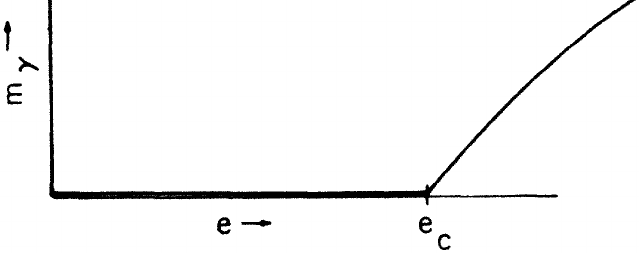
\includegraphics[width=0.42\textwidth]{fig1}
  \refstepcounter{figure}%
  \caption*{Fig. 1. Speculative plot of photon mass vs renormalized
    charge $e$, in unknown units. The transition at $e_{c}$ is
    second-order (see text).}
  \label{fig:1}
\end{figure}

By analogy with the solid-state situation one can think of the
transition from zero to nonzero photon mass as a change of phase: this
analogy is best understood by imagining the particles of quantum
electrodynamics to be the excitations of a medium (the ether).  In this
case it is the ether which undergoes a change of phase at $e_{c}$.  There
is again a question whether this change of phase is first-order (cf.\
Fig.~\ref{fig:2}) or second-order (Fig.~\ref{fig:1}).  (Coleman and
Weinberg${}^{7}$ have found a nontrivial example of a first-order
transition in another context.)

The model discussed in this paper is a single Abelian gauge field
coupled (with strength $g$) to massive quarks.  In weak coupling the
gauge field behaves like a normal free zero-mass field (despite
modifications introduced in the lattice quantization) and the quarks are
unbound.  In strong coupling the gauge field is massive and the quarks
are bound, showing the existence of the second phase.  Thus there should
be a phase transition at some intermediate value of $g$.  Nothing is
known about this transition at the present time.

\begin{figure}[t]
  \centering
  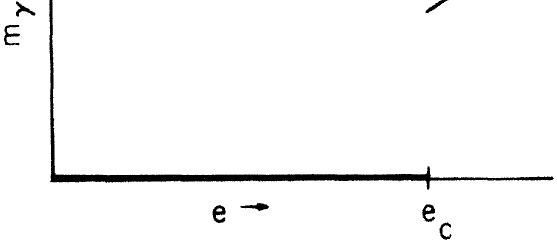
\includegraphics[width=0.42\textwidth]{fig2}
  \refstepcounter{figure}%
  \caption*{Fig. 2. Speculative plot of photon mass vs renormalized
    charge $e$ if there is a first-order transition at $e_{c}$.}
  \label{fig:2}
\end{figure}

The quantization procedure and strong-coupling approximation described
in this paper can be applied to non-Abelian gauge theories also.  This
will be explained briefly in Sec.~III.

An extraordinary feature of the strong-coupling expansion of the lattice
theory (see Sec.~IV) is that it has the same general structure as the
relativistic string models of hadrons.${}^{8}$  The vacuum expectation
values of the gauge theory involve (in the strong-coupling expansion)
sums over all quark paths and sums over all surfaces connecting these
paths; the surfaces are generated by the gauge field treated in strong
coupling.  The paths and surfaces are defined on a discrete lattice.
There are geometrical difficulties in relating the surfaces on the
lattice to the continuum surfaces of the string models; it is not known
at present whether these difficulties can be overcome.

In Sec.~II the nature of the quark binding mechanism will be discussed,
qualitatively.  In Sec.~III the gauge theory will be formulated on a
discrete lattice, both classically and quantum mechanically.  In
Sec.~IV the strong-coupling expansion for the lattice gauge theory is
explained.  In Sec.~V a cursory discussion of weak coupling is given.
In Sec.~VI there is a brief discussion of the problem of Lorentz
invariance and the relation to string models.

% =====================================================================
%  Section II. Quark Binding Mechanism
% =====================================================================
\section{QUARK BINDING MECHANISM}\label{sec:binding}

The binding mechanism will be explained in this section using the
Feynman path-integral picture.  The path-integral framework will be used
in an intuitive rather than a formal way.  Consider the current-current
propagator
\begin{equation}
D_{\mu\nu}(x) = \ev{\mathrm{T}\,J_{\mu}(x)J_{\nu}(0)}\,,
\label{eq:2.1}
\end{equation}
whose Fourier transform determines the $e^{+}e^{-}$ annihilation cross
section into hadrons.  Assume that the currents $J_{\mu}(x)$ are built
from quark fields as in the quark-parton model.  Assume that the quarks
interact through a single gauge field.  (The restriction to one field is
only for simplicity.)  In the Feynman path-integral picture the
propagator $D_{\mu\nu}(x)$ is given by a weighted average over all
possible classical quark paths and all possible classical values of the
gauge field.  The currents $J_{\mu}(x)$ and $J_{\nu}(0)$ are thought of
as producing a quark pair at the origin which later annihilate at the
point $x$:  One has to sum over all paths joining the points $0$ and $x$
for each of the pair of quarks.

An example of paths for the quark and antiquark are shown in
Fig.~\ref{fig:3}.  The vacuum can also emit and absorb quark pairs; this
leads to further closed loops as illustrated in Fig.~\ref{fig:4}.  All
possible loops must be summed over too.  It is also possible to have
independent loops for the points $0$ and $x$ (Fig.~\ref{fig:5}), but
this possibility will not be important here.

\begin{figure}[t]
  \centering
  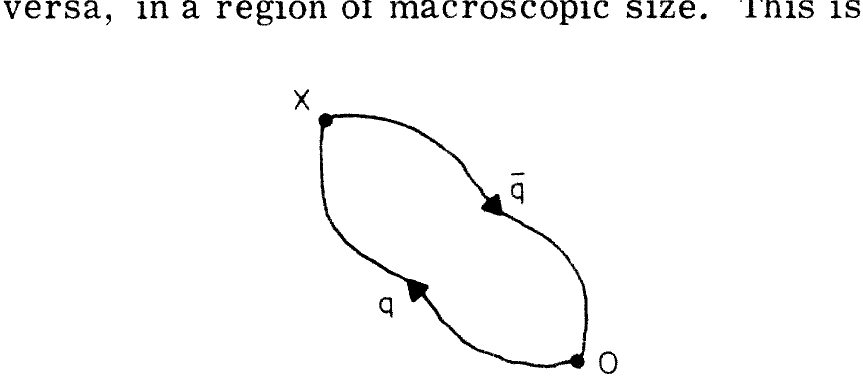
\includegraphics[width=0.52\textwidth]{fig3}
  \refstepcounter{figure}%
  \caption*{Fig. 3. An example of quark ($q$) and antiquark ($\bar q$)
    paths connecting the points $0$ and $x$.}
  \label{fig:3}
\end{figure}

\begin{figure}[t]
  \centering
  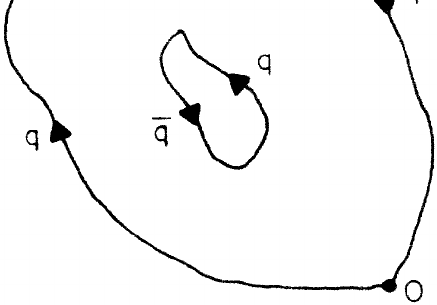
\includegraphics[width=0.5\textwidth]{fig4}
  \refstepcounter{figure}%
  \caption*{Fig. 4. Example of current loop (as in Fig. 3) with extra
    vacuum loop.}
  \label{fig:4}
\end{figure}

The weight associated with a given quark path or set of paths includes a
factor of $\exp[ig\oint A_{\mu}(x)\,ds^{\mu}]$, where $A_{\mu}(x)$ is
the gauge field.  Here $\oint ds^{\mu}$ is a line integral or a sum over
line integrals for each of the quark-antiquark loops, including the loop
joining the points $0$ and $x$.  The constant $g$ is the coupling
constant of the gauge theory.  There are further weight factors
independent of $A$.  Finally, independently of the quark paths there is
another weight factor, namely, the exponential of the free action for
the gauge field.  The combined weight factor is then averaged over all
quark paths and all gauge fields $A_{\mu}(x)$ to give the current-current
propagator.

\begin{figure}[t]
  \centering
  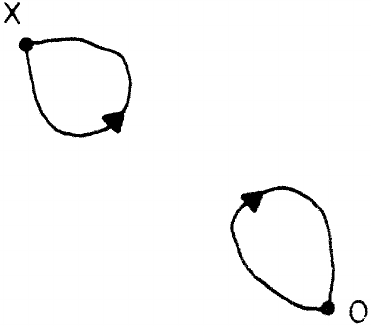
\includegraphics[width=0.42\textwidth]{fig5}
  \refstepcounter{figure}%
  \caption*{Fig. 5. Example of separate quark loops for the points $0$
    and $x$. (Integration over the gauge field produces gauge
    propagators which connect these loops.)}
  \label{fig:5}
\end{figure}

In order that quarks exist as separate final-state particles it must be
possible to have quark-antiquark loops with well-separated quark and
antiquark lines, at least when $x$ and $0$ are far apart.  This is
illustrated in Fig.~\ref{fig:6}(a).  If the quark and antiquark paths
are unlikely to separate beyond a fixed size, say $10^{-13}$~cm [see
Fig.~\ref{fig:6}(b)], then clearly no detector will see a quark or
antiquark in isolation.

It is assumed in this discussion that vacuum loops are not important.
If vacuum loops are important enough then space will be filled with a
high density of vacuum-produced quark-antiquark pairs.  In particular,
there will be many quark-antiquark pairs inside a detector of
macroscopic size.  The question then is whether there can be an excess
of quarks over antiquarks, or vice versa, in a region of macroscopic
size.  This is a more difficult question to answer and will not be
discussed in this paper.

\begin{figure}[t]
  \centering
  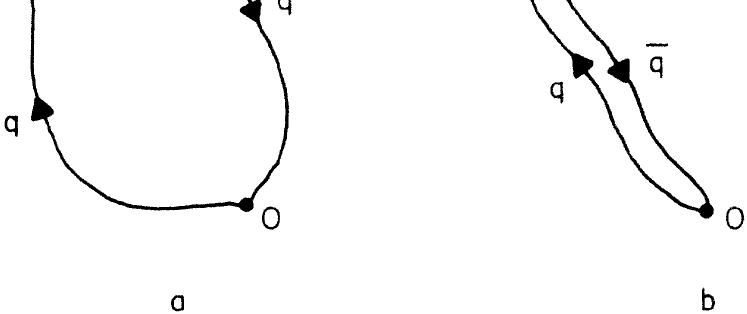
\includegraphics[width=0.55\textwidth]{fig6}
  \refstepcounter{figure}%
  \caption*{Fig. 6. (a) Loop with well-separated quark and antiquark.
    (b) Loop with small separation between quark and antiquark.}
  \label{fig:6}
\end{figure}

Note that $x$ must be large:  If $x$ is small there is little likelihood
of finding a large size loop.  This may seem a bit peculiar:  One expects
quarks to appear in the final state of $e^{+}e^{-}$ annihilation only at
large virtual-photon momentum $q$ if they appear at all, and large $q$
means small $x$, not large $x$.  The answer to this paradox has two
parts.  First, the important paths in the Feynman path integral bear no
detailed relation to possible physical final states (the paths are paths
of bare particles, not physical particles).  Secondly, large $x$ does
not necessarily mean small $q$.  In fact the study of whether
well-separated quark-antiquark paths exist for large $x$ is really a
search for a quark-antiquark threshold in $e^{+}e^{-}$ annihilation,
which would contribute a term $\sim \exp(2imx)/x^{p}$ to the
current-current propagator for large $x$, where $m$ is the quark mass.
(Here $\sim$ means up to a power of $x$.${}^{9}$)  Such a term
corresponds in momentum space to the singularity at the threshold
$q^{2} = (2m)^{2}$.

Suppose the gauge-field averaging is performed before the quark-paths
averaging.  Then one determines the average over all gauge fields of the
weight factor $\exp[ig\oint A_{\mu}(y)\,ds^{\mu}]$ weighted further with
the exponential of the free gauge-field action.  For an Abelian gauge
theory this average can be computed explicitly:  It is
\[
  \exp\!\Big[-g^{2}\oint\!\!\oint ds^{\mu}\,ds'^{\nu}\,D_{\mu\nu}(y-y')\Big],
\]
where $D_{\mu\nu}(y-y')$ is the free gauge-field propagator.

The quark binding mechanism can be seen by comparing the above
expression for one space dimension and three space dimensions.  In three
space dimensions this calculation gives no binding (the binding occurs
only with a modified gauge-field action:  see Sec.~IV), while there is
binding in one space dimension.  In three space dimensions
$D_{\mu\nu}(y-y')$ behaves as $(y-y')^{-2}$.  In consequence large
values of $(y'-y)$ are negligible in the double line integral.  Hence,
the double integral is proportional to $P$, where $P$ is the length of
the loop.  Unfortunately the integral is divergent at $y'=y$; a cutoff
is needed for the integral to make sense.  Since a cutoff will be
introduced anyway in this paper, this is not a major concern.  For
simple loops, the perimeter $P$ is roughly of order $(x^{2})^{1/2}$
(ignoring the case that $x$ is close to the light cone).  Thus one has
an exponential of the type one expects when free quarks are present.

In one space dimension, $D_{\mu\nu}(y-y')$ behaves as
$\ln[(y-y')^{2}]$ for $y'-y$ large, and $y'$ and $y$ can freely range
separately over the loop.  In this case the double integral is
proportional to $P^{2}$.  Now the gauge-field average behaves as
$e^{-cP^{2}}$ where $c$ is a constant.  In this case the contribution of
large loops is heavily suppressed and there are no free quarks.  [The
case of nearby quark-antiquark pairs as in Fig.~\ref{fig:6}(b) is
special --- in this case large $y-y'$ is unimportant due to cancellation
between the quark path and the nearby and oppositely directed antiquark
path.  In this case the double integral behaves as $P$, not $P^{2}$, but
in this case there are no isolated quarks.]

In the strongly coupled lattice gauge theory described in later
sections, the gauge-field average of $\exp[ig\oint A_{\mu}(x)\,ds^{\mu}]$
behaves as $\exp(-cA)$, where $A$ is the enclosed area of the loop.
This heavily suppresses large loops, such as in Fig.~\ref{fig:6}(a),
where $A$ is of order $P^{2}$.  One can think of one factor $P$ as being
roughly $(x^{2})^{1/2}$, the other $P$ as being analogous to a mass
multiplying $(x^{2})^{1/2}$.  Since $P \to \infty$ as $x \to \infty$,
the quark-antiquark threshold is at infinite mass.

\begin{figure}[t]
  \centering
  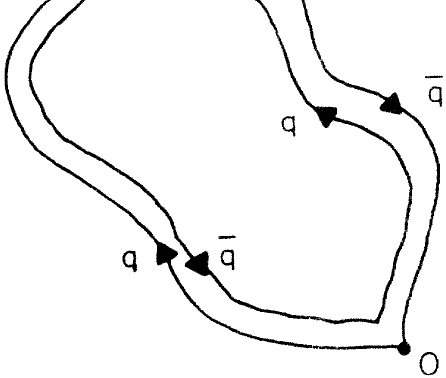
\includegraphics[width=0.42\textwidth]{fig7}
  \refstepcounter{figure}%
  \caption*{Fig. 7. Quark-antiquark loop with nearby vacuum loop.}
  \label{fig:7}
\end{figure}

In all these calculations one can have a large loop if there is a nearby
vacuum loop (Fig.~\ref{fig:7}).  In this case one always gets
$e^{-cP}$ behavior.  For example, in the strong-coupling case the
relevant enclosed area is the area between the two loops which is
proportional to the perimeter $P$ provided the separation of the two
loops is fixed independently of $P$.  This is in accord with Schwinger's
picture.  While an isolated well-separated loop may be suppressed (due
to $P^{2}$ or $A$ dependence in the exponential) a loop closely shielded
by a vacuum-polarization loop is always unsuppressed.

The binding mechanism proposed here is soft:  The exponential damping is
associated with large size loops having large areas.  The behavior of
small loops is irrelevant to the binding mechanism.  Also for small
loops both their area and perimeter are small and neither is of great
importance in an exponential.

The mechanism discussed here works equally well for Dirac quarks or
scalar quarks.  This is in contrast to the Higgs mechanism which can
wipe out the charge of scalar particles only.

% =====================================================================
%  Section III. Lattice Quantization of Gauge Fields
% =====================================================================
\section{LATTICE QUANTIZATION OF GAUGE FIELDS}\label{sec:lattice}

\subsection{Classical action on a lattice}\label{sec:classical}

In this section the gauge-field action (space-time integral of the
Lagrangian) will be defined on a discrete lattice with spacing $a$ in
Euclidean space-time.  The simplest way to proceed is to consider a
continuum action, substitute finite-difference approximations for
derivatives, and replace the space-time integral by a sum over the
lattice sites.  However, the result of this is an action which is not
gauge-invariant for nonzero $a$.  Because of the vagaries of
renormalization this is likely to mean that the quantized theory still
lacks gauge invariance in the limit $a \to 0$ (if such a limit exists).
The alternative is to formulate gauge invariance for a lattice theory,
and tinker with the action so that it is gauge invariant for any $a$.
This alternative will be pursued here.

For convenience a charged Dirac field $\psi$ coupled to a single gauge
field $A_{\mu}$ will be discussed in detail.  Generalizations to
non-Abelian gauge groups will be noted later.

On the lattice the fields are $\psi_{n}$, $\bar\psi_{n}$, and
$\thl{\mu\nu}(n)$, where $n$ is a four-vector with integer components
referring to points on a simple hypercubic lattice.

A simple action on the lattice for the Dirac field (ignoring the gauge
field for now) has the form
\begin{equation}
A_{D} = -a^{3}\sum_{n} m_{b}\bar\psi_{n}\psi_{n}
        + a^{3}\sum_{n,\mu} \bar\psi_{n}\gamma_{\mu}
          \frac{\psi_{n+\hat\mu}-\psi_{n-\hat\mu}}{2a},
\label{eq:3.1}
\end{equation}
where $m_{b}$ is the bare mass; $\hat\mu$ is a unit vector along the axis
$\mu$; $a^{3}\sum_{n}$ replaces the space-time integration of the
continuum theory, and $(\psi_{n+\hat\mu}-\psi_{n-\hat\mu})/2a$ replaces
$\partial_{\mu}\psi$.  There is no over-all factor of $i$ due to the
Euclidean metric.  A gauge transformation on the lattice can be defined
as follows.
\begin{equation}
\psi_{n} \to e^{i\Lambda_{n}}\psi_{n},\qquad
\bar\psi_{n} \to \bar\psi_{n}e^{-i\Lambda_{n}},
\label{eq:3.2}
\end{equation}
\begin{equation}
\thl{\mu\nu}(n) \to \thl{\mu\nu}(n) - \frac{\gamma_{n+\hat\mu}-\gamma_{n}}{a},
\label{eq:3.3}
\end{equation}
\stepcounter{equation}%   % the paper has no Eq. (3.4)
where $g$ is the coupling constant and $\gamma_{n}$ is arbitrary.  The
terms $\bar\psi_{n}\psi_{n+\hat\mu}$ and $\bar\psi_{n+\hat\mu}\psi_{n}$
are not invariant to this transformation; the corresponding
gauge-invariant expressions are
$\bar\psi_{n}\psi_{n+\hat\mu}\exp(iga\,\thl{\mu\nu}(n))$ and
$\bar\psi_{n}\psi_{n+\hat\mu}\exp(-iga\,\thl{\mu\nu}(n))$.  Thus, a
gauge-invariant form for $A_{D}$ is
\begin{equation}
\begin{split}
A_{D} = {} & -a^{3}\sum_{n} m_{b}\bar\psi_{n}\psi_{n}\\
           & + \frac{a^{2}}{2}\sum_{n,\mu}
             \Bigl[\bar\psi_{n}\gamma_{\mu}\psi_{n+\hat\mu}
             e^{iga\,\thl{\mu\nu}(n)}
             -\bar\psi_{n+\hat\mu}\gamma_{\mu}\psi_{n}
             e^{-iga\,\thl{\mu\nu}(n)}\Bigr].
\end{split}
\label{eq:3.5}
\end{equation}

In the action $A_{D}$, the field $\thl{\mu\nu}$ acts like an angular
variable:  $A_{D}$ is periodic in $\thl{\mu\nu}$ with period $2\pi$.

The free gauge-field action will be defined to preserve this property.
This does not mean that $\thl{\mu\nu}$ is an angular variable in the
continuum limit.  Owing to the relation~\eqref{eq:3.6},
$\thl{\mu\nu}$ becomes an infinitesimal angular variable $A_{\mu}(x)$
for $a \to 0$; such a variable has the range
$-\infty < A_{\mu}(x) < \infty$ without any periodicity.
\begin{equation}
\thl{\mu\nu}(n) = a\,g\,A_{\mu}(na) + \order{a^{2}}.
\label{eq:3.6}
\end{equation}

A gauge-invariant lattice approximation for $F_{\mu\nu}$ is
\begin{equation}
F_{\mu\nu}(n) =
\frac{\thl{\mu\nu}(n)-\thl{\nu\mu}(n)-\thl{\mu\nu}(n+\hat\nu)
+\thl{\nu\mu}(n+\hat\mu)}{a}.
\label{eq:3.7}
\end{equation}

It is convenient to define a rescaled form of $\thl{\mu\nu}$:
\begin{equation}
f_{\mu\nu}(n) = \thl{\mu\nu}(n)+\thl{\nu\mu}(n+\hat\mu)
-\thl{\mu\nu}(n+\hat\nu)-\thl{\nu\mu}(n).
\label{eq:3.8}
\end{equation}

A simple lattice action for the gauge field which preserves periodicity
is
\begin{equation}
A_{G} = \frac{1}{2g^{2}}\sum_{n,\mu\nu}
        \Bigl[1-\tfrac{1}{2}\bigl(e^{if_{\mu\nu}(n)}+e^{-if_{\mu\nu}(n)}\bigr)\Bigr].
\label{eq:3.9}
\end{equation}

In the continuum limit, $f_{\mu\nu} \to 0$ due to the factor $a$ in the
definition of $f_{\mu\nu}$.  Thus for small $a$, one can write
\[
A_{G} = \frac{1}{2g^{2}}\sum_{n,\mu\nu}
        \Bigl[\tfrac{1}{4}\bigl(f_{\mu\nu}(n)\bigr)^{2}+\cdots\Bigr],
\]
The constant term is irrelevant.  The linear term in $f_{\mu\nu}$ is 0
because $f_{\mu\nu}$ is odd in the indices $\mu$ and $\nu$.  The
quadratic term gives
\stepcounter{equation}%   % the paper has no Eq. (3.10)
\begin{equation}
A_{G} = -\frac{1}{2g^{2}}\,a^{4}\sum_{n,\mu\nu}\bigl(F_{\mu\nu}(n)\bigr)^{2},
\label{eq:3.11}
\end{equation}
which is the conventional gauge-field action in a lattice approximation.
The terms involving $f_{\mu\nu}^{3}$, $f_{\mu\nu}^{4}$, etc.\ all vanish
for $a\to0$ even after removing a factor $a^{4}$ to convert
$\sum_{n}$ into an integral.

The full action may now be written
\begin{equation}
\begin{split}
A = {} & -\epsilon\sum_{n}\bar\psi_{n}\psi_{n}
         + \kappa\sum_{n,\mu}\Bigl[
           \bar\psi_{n+\hat\mu}\gamma_{\mu}\psi_{n}e^{i\thl{\mu\nu}(n)}
           -\bar\psi_{n}\gamma_{\mu}\psi_{n+\hat\mu}e^{-i\thl{\mu\nu}(n)}\Bigr]\\
       & + \frac{1}{2g^{2}}\sum_{n,\mu\nu}
         \Bigl[1-\tfrac{1}{2}\bigl(e^{if_{\mu\nu}(n)}+e^{-if_{\mu\nu}(n)}\bigr)\Bigr],
\end{split}
\label{eq:3.12}
\end{equation}
with $\epsilon = m_{0}a^{4}$, $\kappa = a^{2}/2$.  This action reduces
to the usual continuum action for $a \to 0$; for finite $a$ it is gauge
invariant and periodic in the gauge field.  Note, however, that the
continuum limit is a classical limit in which the lattice variables
$\psi_{n}$, $\bar\psi_{n}$, and $\thl{\mu\nu}$ approach continuum
functions $\psi(x)$, $\bar\psi(x)$, and $A_{\mu}(x)$ with $x=na$.  The
continuum limit of the quantized theory is much harder to discuss owing
to renormalization problems.

\subsection{Quantization}\label{sec:quantization}

The problem of principal interest here is the quantization of the gauge
field.  Therefore, the gauge field will be quantized by itself to start
with.  Later the quantization of $\psi$ will be discussed.  At the end of
this section the generalizations to non-Abelian gauge theories will also
be described.

The quantization of the lattice gauge theory will be carried out in two
steps.  The first step will be to define a lattice version of Euclidean
vacuum expectation values, starting from a lattice version of the Feynman
path integral.  The second step will be to define a quantum theory on the
lattice, which will allow the introduction of a real time variable and the
definition of particle states and scattering amplitudes.  In both cases
the lattice provides an ultraviolet cutoff and there is no Lorentz
invariance.  Lorentz invariance can only be achieved in the limit
$a$ (lattice spacing) $\to 0$, if at all, and in practice this is a
difficult limit to evaluate.

As discussed in Sec.~\ref{sec:intro}, one would like to calculate the
gauge-field average of $\exp[ig\oint A_{\mu}(x)\,ds^{\mu}]$ weighted
with the gauge-field action.  On a lattice the line integral becomes a
sum over a closed path $P$ on the lattice (see, e.g.,
Fig.~\ref{fig:8}).  The sum has the form $ig\sum_{P}(\pm)\thl{\mu\nu}$,
where a particular $\thl{\mu\nu}$ is present in the sum if the path
connects the sites $n$ and $n+\hat\mu$ ($-\thl{\mu\nu}$ appears if the
path goes from $n+\hat\mu$ to $n$).

\begin{figure}[t]
  \centering
  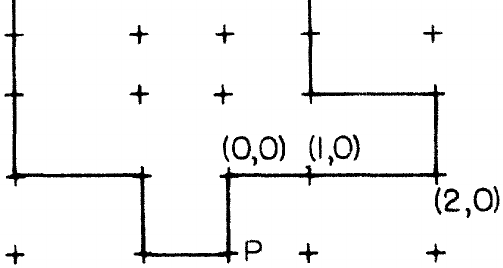
\includegraphics[width=0.4\textwidth]{fig8}
  \refstepcounter{figure}%
  \caption*{Fig. 8. Example of a lattice path $P$.}
  \label{fig:8}
\end{figure}

On the lattice, an average over all gauge fields involves integrating
over all values of the $\thl{\mu\nu}$ for all $n$ and $\mu$.  Normally
one would have integrals over an infinite range:
$-\infty < \thl{\mu\nu} < \infty$, but because of the periodicity in
$\thl{\mu\nu}$ there is no point to integrating over more than a single
period.  Thus the lattice version of the gauge-field average is
\begin{equation}
I_{\theta}(P) = \prod_{n,\mu\nu}\int\ddth{\mu\nu}
  \exp\!\Bigl[i\sum_{P}(\pm)\thl{\mu\nu}
    +\frac{1}{2g^{2}}\sum_{n,\mu\nu}
      \bigl(e^{if_{\mu\nu}(n)}+e^{-if_{\mu\nu}(n)}\bigr)\Bigr].
\label{eq:3.13}
\end{equation}
\begin{equation}
Z_{\theta} = \prod_{n,\mu\nu}\int\ddth{\mu\nu}
  \exp\!\Bigl[\frac{1}{2g^{2}}\sum_{n,\mu\nu}
    \bigl(e^{if_{\mu\nu}(n)}+e^{-if_{\mu\nu}(n)}\bigr)\Bigr].
\label{eq:3.14}
\end{equation}

Note that no gauge-fixing term has been added to the action.  The finite
range of $\thl{\mu\nu}$ makes a gauge-fixing term unnecessary.  In
continuum gauge theories where $A_{\mu}(x)$ has an infinite range
$[-\infty < A_{\mu}(x) < \infty]$ a gauge-fixing term is essential to
have a convergent functional integral.  The reason for this is that the
volume in path-integral space generated by all possible gauge
transformations is infinite; the gauge-fixing term provides a convergence
factor in this volume.  In the lattice theory the total volume of
integration is finite if the lattice itself is of finite extent; no
convergence factor is required.  For a lattice of infinite extent there
are divergences due to the infinite number of integrations (in other
words, the infinite lattice volume), but these divergences are normally
removed by the division by $Z$ (this division is equivalent to removing
all vacuum loops in perturbation theory).

One can define more conventional vacuum expectation values in a similar
manner.  For instance, one can define a propagator.  In the absence of a
gauge-fixing term it is awkward to define a propagator for the gauge
field $\thl{\mu\nu}$ itself; instead one can define a gauge-invariant
propagator as
\begin{equation}
D_{\mu\nu}(n) = Z_{\theta}^{-1}\prod_{m,\rho}\int\ddth{\rho\sigma}
  e^{i\thl{\mu\nu}(n)}e^{-i\thl{\mu\nu}(0)}
  \exp\!\Big[\tfrac{1}{2g^{2}}\sum_{m,\rho\sigma}
    \bigl(e^{if_{\rho\sigma}(m)}+e^{-if_{\rho\sigma}(m)}\bigr)\Big].
\label{eq:3.15}
\end{equation}
This is a propagator for the operator $e^{i\thl{\mu\nu}}$; it is defined
only for the lattice points $n$ of a Euclidean space-time lattice.  If
the lattice spacing is $a$, this means the propagator is defined only for
imaginary times of the form $in_{0}a$, where $n_{0}$ is an integer.

A theory defined only for discrete imaginary values of the time leaves
much to be desired.  Fortunately, one can generalize the theory to define
a Hamiltonian for a quantized theory.  The particle eigenstates and
scattering amplitudes of the theory can then be obtained, in principle,
by diagonalizing the Hamiltonian.  The Hamiltonian will be defined using
the transfer-matrix formalism.  Only a brief discussion of the
transfer-matrix approach will be given here.  For a review${}^{6}$ of the
ideas see Wilson and Kogut.${}^{6}$  A detailed discussion including
approximate calculation of single-particle energies and scattering
amplitudes in a simple scalar field theory is given by Suri.${}^{5}$

Consider the expression for $Z$.  Introduce finite bounds on the lattice
coordinate $n_{0}$, say
\begin{equation}
-N \le n_{0} \le N.
\label{eq:3.16}
\end{equation}
Introduce periodic boundary conditions (see below${}^{6}$).  Then one can
write $Z$ as the trace of a matrix $V$, more precisely
\begin{equation}
Z = \Tr V^{2N+1}.
\label{eq:3.17}
\end{equation}
This formula is made possible by the fact that each term in the action
$A$ involves no more than two adjacent values of $n_{0}$.

To set up the matrix $V$, one must first understand the space on which it
acts.  The space used here is the space of all functions
$\Phi(\thl{ij})$ (periodic in each $\thl{ij}$ with period $2\pi$), where
the index $i$ runs from 1 to 3 only, and the lattice variable $n$ has
only three components $(n_{1},n_{2},n_{3})$.  The matrix $V$ will be
defined as a function of two sets of arguments, say $\thl{ij}$ and
$\thl{ij}'$, these two sets of arguments referring to the space-time
fields $\thl{ij}$ for two adjacent values of $n_{0}$.  Matrix
multiplication of two $V$'s involves integrations over a set of variables
$\thl{ij}$.  Define $V$ as
\begin{equation}
V = \prod_{n}\prod_{i,j}\int\ddth{i0}\,e^{U}.
\label{eq:3.18}
\end{equation}

The quantity $U$ as written out below looks complicated, but all it is is
that part of the action $A$ referring to a given nearest-neighbor pair of
values for $n_{0}$; terms in $A$ referring to a single value of $n_{0}$
are divided equally between the matrices connecting $n_{0}$ to
$n_{0}+1$ and $n_{0}$ to $n_{0}-1$.  The result is
\begin{equation}
U = \frac{1}{2g^{2}}\sum_{n,i,j}\Bigl[
    \bigl(e^{if_{0i,j}(n)}+e^{-if_{0i,j}(n)}\bigr)
    +\bigl(e^{i\thl{i0,j}(n)}+e^{-i\thl{i0,j}(n)}\bigr)\Bigr],
\label{eq:3.19}
\end{equation}
where
\begin{equation}
f_{0i}(n) = \thl{0i}(n)+\thl{i0}(n+\hat0)-\thl{0i}(n+\hat i)-\thl{i0}(n),
\label{eq:3.20}
\end{equation}
and
\begin{equation}
f_{i0}(n) = \thl{i0}(n)+\thl{0i}(n+\hat i)-\thl{i0}(n+\hat0)-\thl{0i}(n).
\label{eq:3.21}
\end{equation}

With the definition of $V$ given here, the trace $\Tr V^{2N+1}$ is easily
seen to reproduce all the integrations involved in the equation for $Z$,
and the sum of the $2N+1$ exponents $U$ reproduces the action $A$ except
for some additional terms coupling the boundary $n_{0}=N$ to the
boundary $n_{0}=-N$ to achieve a periodic structure.

Note that the 0 components of $\thl{\mu\nu}$ have received special
treatment.  This is because there are no terms in $A$ involving
$\thl{0\mu}$ for more than one value of $n_{0}$; this makes it possible
to include integrations over $\thl{0\mu}$ in the definition of $V$
rather than in the definition of matrix multiplication.

The matrix $V$ is used to define the quantized theory.  Briefly, this is
accomplished as follows.  $V$ is a Hermitian matrix, i.e.,
\begin{equation}
V(\theta,\theta')^{*} = V(\theta',\theta).
\label{eq:3.22}
\end{equation}
[This result can be verified by close examination of
Eqs.~\eqref{eq:3.18}--\eqref{eq:3.21}.  One must remember that the
variables $\thl{0\mu}$ are integrated out in the definition of $V$.  This
means that in forming the complex conjugate of $V$ one can also make the
change of variable $\thl{0\mu} \to -\thl{0\mu}$.]  Hence $V$ has a
complete orthogonal set of eigenstates $\psi_{\lambda}$ and eigenvalues
$\lambda$.  The Hamiltonian $H$ is now defined as follows:  The
eigenstates of $H$ are the eigenstates of $V$; the eigenvalues of $H$ are
given by
\begin{equation}
E_{\lambda} = -a^{-1}\ln\lambda,
\label{eq:3.23}
\end{equation}
where $\lambda$ is the corresponding eigenvalue of $V$.  The reason for
the factor $a^{-1}$ will be evident shortly.  The reason for using the
logarithm is so that the energies of multiparticle scattering states will
be the sum of single-particle energies (see Suri${}^{5}$).

A problem arises with this definition if $V$ has any negative eigenvalues
$\lambda$.  If this were to happen, $H$ would have complex eigenvalues.
This did not happen in the case studied by Suri${}^{5}$; whether it
happens here the author does not know; this question must be studied
further.  Even if $V$ has negative eigenvalues, they may be irrelevant in
the limit $a\to0$ if such a limit exists.

The definition~\eqref{eq:3.23} means that
\begin{equation}
V = e^{-aH}.
\label{eq:3.24}
\end{equation}
This means $V$ is the operator which propagates a state through an
imaginary time $ia$.  It is a consequence of this that the propagator
$D_{\mu\nu}$ is a vacuum expectation value for imaginary time $in_{0}a$
in the theory with Hamiltonian $H$.  For proof of this statement see
Refs.~5 and~6.

The lattice quantization procedure can be extended to non-Abelian gauge
theories.  This is done as follows.  In place of the single variable
$\thl{\mu\nu}$, one has a set of variables $\thl{\mu\nu}^{a}$ where $a$
is an internal index.  For each $n$ and $\mu$, $\thl{\mu\nu}$ is to
parametrize an element $h_{\mu\nu}$ of the gauge group.  In place of
$\exp(i\thl{\mu\nu})$ one substitutes $U(\thl{\mu\nu})$, where $U$ is the
unitary matrix representing $\thl{\mu\nu}$ in the quark representation.
The product $\bar\psi_{n}\gamma_{\mu}\psi_{n+\hat\mu}\exp(i\thl{\mu\nu})$
is replaced by $\bar\psi_{n}\gamma_{\mu}U(\thl{\mu\nu})\psi_{n+\hat\mu}$.
A gauge transformation is defined by a set of group transformations
$\gamma_{n}$; under these transformations
\begin{equation}
\thl{\mu\nu} \to \thl{\mu\nu}^{a},
\label{eq:3.25}
\end{equation}
\begin{equation}
h_{\mu\nu} = \exp\!\Bigl(i\sum_{a}T^{a}\thl{\mu\nu}^{a}\Bigr),
\label{eq:3.26}
\end{equation}
\begin{equation}
\psi_{n} \to U(\gamma_{n})\psi_{n},\qquad
\bar\psi_{n} \to \bar\psi_{n}U(\gamma_{n})^{-1},
\label{eq:3.27}
\end{equation}
\begin{equation}
U(\thl{\mu\nu}) \to U(\gamma_{n})\,U(\thl{\mu\nu})\,U(\gamma_{n+\hat\mu})^{-1},
\label{eq:3.28}
\end{equation}
where $\gamma_{n}\,\thl{\mu\nu}\,\gamma_{n+\hat\mu}^{-1}$ is computed
according to the multiplication law of the group.  A simple
gauge-invariant action for the gauge field is
\begin{equation}
\begin{split}
A_{G} = \frac{1}{2g^{2}}\sum_{n,\mu\nu}\Bigl[1-\tfrac{1}{2}\Tr
    &\bigl(U(\thl{\mu\nu}(n))\,U(\thl{\nu\mu}(n+\hat\mu))\\
    &\qquad U^{-1}(\thl{\mu\nu}(n+\hat\nu))\,U^{-1}(\thl{\nu\mu}(n))\bigr)\Bigr],
\end{split}
\label{eq:3.29}
\end{equation}
where the unitary transformation $U_{A}$ is taken from the adjoint
representation of the group.  (Any representation will do as well.)  In
the classical continuum limit, $\thl{\mu\nu}$ becomes an infinitesimal
group transformation $\thl{\mu\nu} = ga\,A_{\mu}^{a}(na)T^{a}$ with
$A_{\mu}^{a}$ fixed as $a\to0$; in this limit one can show, with some
effort, that $A_{G}$ reduces to the standard continuum Yang-Mills action.
When the non-Abelian theory is quantized, the integrations over
$\thl{\mu\nu}$ are group integrations over all elements of the group.
These are compact integrations (for compact groups) and no gauge-fixing
term is required.

Since quark binding can be illustrated using Abelian theory, the
non-Abelian theory will not be studied further.

Finally, the quantization of the Dirac field will be discussed.  It is
convenient initially to quantize the Dirac field in an analogous manner
to the gauge field.  The only problem that occurs is to define
``integration'' for a Fermi field.  This can be done.${}^{11}$

The property of the integral that is crucial for quantization is
translational invariance in the integration variable.  For example, when
quantizing a scalar field $\phi$ on a lattice the field averaging
involves the integral $\int\dd\phi_{n}$ which has the translational
invariance
\begin{equation}
\int\dd\phi_{n}\,f(\phi_{n}+\xi_{n}) = \int\dd\phi_{n}\,f(\phi_{n})
\label{eq:3.30}
\end{equation}
for any integrable function $f$ and any constant $\xi_{n}$.  It is this
translational invariance that makes the Feynman path integral provide a
realization of Schwinger's action principle (see, e.g., Ref.~12 for
further discussion).  Analogously one needs to define an integration over
Fermi fields with the same translational invariance.  Stated abstractly,
one wants to define a bracket operation $(\ )$ defined on functions of
purely anticommuting Fermi fields $\psi_{n}$ with the property
\begin{equation}
(f) = \int f(\psi,\bar\psi)\,\prod_{n}\dd\psi_{n}\,\dd\bar\psi_{n},
\label{eq:3.31}
\end{equation}
where $\psi_{n}$ and $\bar\psi_{n}$ are anticommuting $c$-numbers (these
have been introduced by Schwinger).  The bracket operation should produce
a number for every function $f$; it should also be a linear operation.
Thus for a finite lattice it is sufficient to specify the bracket
$(\ )$ for all monomials in the $\psi_{n}$ and $\bar\psi_{n}$.  Because of
the anticommutation rules, $\psi_{n}^{2}$ and $\bar\psi_{n}^{2}$ vanish
(more correctly, $\psi_{n\alpha}^{2}$ and $\bar\psi_{n\alpha}^{2}$ vanish
where $\psi_{n\alpha}$ and $\bar\psi_{n\alpha}$ are any component of
$\psi_{n}$ and $\bar\psi_{n}$), therefore, there are only a finite number
of possible monomials.  It is now easy to see that the bracket $(\ )$
must vanish for all products of $\psi$'s and $\bar\psi$'s, except the
product containing all possible $\psi$'s and $\bar\psi$'s.  For example,
suppose there are two lattice sites $0$ and $1$, and $\psi_{n}$ and
$\bar\psi_{n}$ are single component fields.  Then the brackets must be
\begin{equation}
(\psi_{0}\bar\psi_{0}\psi_{1}\bar\psi_{1}) = 1,
\label{eq:3.32}
\end{equation}
where 1 is a constant which was chosen arbitrarily.  This definition of
the bracket operation satisfies translational invariance:  for example,
because the terms multiplying the $\psi$'s are all 0.  Note also that
the anticommutation rules mean that, for example,
\begin{equation}
(\bar\psi_{0}\psi_{0}\bar\psi_{1}\psi_{1}) = -1.
\label{eq:3.33}
\end{equation}
(In analogy to the scalar case, one requires $\psi\bar\psi = 1$, not
$\psi\bar\psi = 1 - \bar\psi\psi$.)

One can now define the Feynman path integral on a lattice for the
complete gauge theory including the Dirac fields.  For example, the
current-current propagator on the lattice is
\begin{equation}
D_{\mu\nu}(x) = Z^{-1}\prod_{n,\rho}\int\dd\psi_{n}\,\dd\bar\psi_{n}\,
  \dd\thl{\rho}\,J_{\mu}(x)J_{\nu}(0)\,e^{A},
\label{eq:3.34}
\end{equation}
where $A$ is the full action of Eq.~\eqref{eq:3.12} and
\begin{equation}
J_{\mu}(n) = \bar\psi_{n}\gamma_{\mu}\psi_{n}.
\label{eq:3.35}
\end{equation}

This formulation of the path integral is different from the formulation
discussed in Sec.~\ref{sec:binding}.  However, one can easily derive a
lattice form of the path integrals of Sec.~\ref{sec:binding} from the
present expression.  The procedure is to expand
Eq.~\eqref{eq:3.34} in powers of $\kappa$, where $\kappa$ is the
coefficient of the nearest-neighbor coupling terms
$\bar\psi_{n}\gamma_{\mu}\psi_{n+\hat\mu}e^{i\thl{\mu\nu}}$ etc.  This
nearest-neighbor coupling term can be represented diagrammatically by a
line from the site $n$ to the site $n+\hat\mu$.  The expansion is best
described by studying an example of a term from the expansion of the
numerator of Eq.~\eqref{eq:3.34}, which will now be discussed.  An
example of a term in the expansion is represented diagrammatically in
Fig.~\ref{fig:9}.  The expression for this term is
\begin{equation}
\begin{split}
D = {} & (-1)\kappa^{4}\,
    e^{i[\thl{\mu\nu}(0,0)+\thl{\mu\nu}(1,0)+\thl{\mu\nu}(0,1)+\thl{\mu\nu}(1,1)]}\\
      & \times \bigl(\bar\psi_{00}\gamma_{\mu}\psi_{10}\bigr)
        \bigl(\bar\psi_{10}\gamma_{\nu}\psi_{11}\bigr)
        \bigl(\bar\psi_{11}\gamma_{\mu}\psi_{01}\bigr)
        \bigl(\bar\psi_{01}\gamma_{\nu}\psi_{00}\bigr),
\end{split}
\label{eq:3.36}
\end{equation}
($D$ for diagram), where the four lattice sites involved are
$(n_{0},n_{1}) = (0,0)$, $(1,0)$, $(0,1)$, and $(1,1)$; the values of
$n_{2}$ and $n_{3}$ are constant and have been suppressed in the notation
of Eq.~\eqref{eq:3.36}.  The action $A_{0}$ omits the $\kappa$ term, and
is
\begin{equation}
A_{0} = -\epsilon\sum_{n}\bar\psi_{n}\psi_{n}
  + \frac{1}{2g^{2}}\sum_{n,\mu\nu}
    \bigl(e^{if_{\mu\nu}(n)}+e^{-if_{\mu\nu}(n)}\bigr).
\label{eq:3.37}
\end{equation}

\begin{figure}[t]
  \centering
  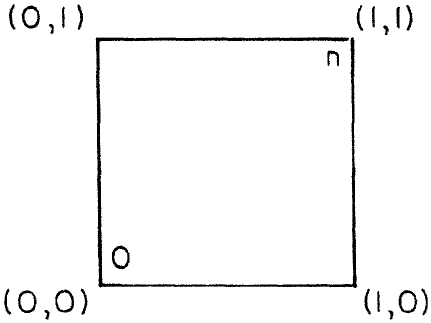
\includegraphics[width=0.3\textwidth]{fig9}
  \refstepcounter{figure}%
  \caption*{Fig. 9. Elementary square on the lattice.}
  \label{fig:9}
\end{figure}

The calculation of $D$ has two parts, one being the integration over all
gauge fields $\thl{\mu\nu}$, the other being the calculation of the
$\psi,\bar\psi$ bracket.  These are independent calculations, i.e., $D$
factors into $D_{\theta}D_{\psi}$.  The quantity $D_{\theta}$ is
\begin{equation}
D_{\theta} = \prod_{n,\mu\nu}\int\ddth{\mu\nu}
  \exp\!\Bigl[i\bigl(\thl{\mu\nu}(0,0)+\thl{\mu\nu}(1,0)
    -\thl{\mu\nu}(1,1)-\thl{\mu\nu}(0,1)\bigr)+A_{0}\Bigr].
\label{eq:3.38}
\end{equation}

This is an example of a gauge-field average of the exponential of a line
integral over a closed loop, the loop being the loop of Fig.~\ref{fig:9}.
The $\psi$ bracket calculation can be factorized further into separate
bracket calculations for each lattice site, since $A_{0}$ contains no
terms involving $\psi$ and $\bar\psi$ coupling different lattice sites.
Consider only the four lattice sites on the loop, for simplicity.  By
moving the $\psi$'s around some (using the anticommuting rule) the
bracket becomes
\[
\begin{split}
&(\bar\psi_{00}e^{-i\thl{\mu\nu}(0,0)}\psi_{00})
 (\bar\psi_{10}e^{-i\thl{\mu\nu}(1,0)}\psi_{10})\\
&\qquad\times
 (\bar\psi_{11}e^{-i\thl{\mu\nu}(1,1)}\psi_{11})
 (\bar\psi_{01}e^{-i\thl{\mu\nu}(0,1)}\psi_{01}).
\end{split}
\]
To make a product of all possible $\psi$'s and $\bar\psi$'s means one
must have products of all possible $\psi_{00}$'s and $\bar\psi_{00}$'s,
all possible $\psi_{10}$'s and $\bar\psi_{10}$'s, etc.  In summary the
complete bracket may be written as a product of four separate brackets.
Define
\begin{equation}
D_{\psi,0} = \bigl(\bar\psi_{00}e^{i\thl{\mu\nu}(0,0)}\psi_{10}\bigr),
\label{eq:3.39}
\end{equation}
\begin{equation}
D_{\theta,0} = \bigl(\bar\psi_{10}\psi_{10}\bigr)_{0}.
\label{eq:3.40}
\end{equation}
Both $D_{\theta}$ and $D_{\psi}$ are matrices in spin space due to the
spinor indices implied for $\psi_{10}$, $\bar\psi_{10}$, $\psi_{00}$,
$\bar\psi_{00}$, and the $\gamma$ matrices.  The full bracket is simply
\begin{equation}
D_{\psi} = -\kappa^{4}\Tr\bigl(D_{\psi,0}\gamma_{\mu}
  D_{\psi,0}\gamma_{\nu}D_{\psi,0}\gamma_{\mu}D_{\psi,0}\gamma_{\nu}\bigr).
\label{eq:3.41}
\end{equation}

The matrices $D_{\psi,0}$ and $D_{\theta,0}$ are easily determined.  For
example, $D_{\theta,0}$ explicitly is
\begin{equation}
D_{\theta,0} = \delta_{\alpha\beta}
  - \epsilon\bigl(\gamma_{0}\gamma_{0}\bigr)_{\alpha\beta}
  - \epsilon\bigl(\gamma_{1}\gamma_{1}\bigr)_{\alpha\beta}
  - \epsilon\bigl(\gamma_{2}\gamma_{2}\bigr)_{\alpha\beta}
  - \epsilon\bigl(\gamma_{3}\gamma_{3}\bigr)_{\alpha\beta}.
\label{eq:3.42}
\end{equation}
The exponential can be expanded in powers of $\epsilon$; assuming the
spinors have four components only the $\epsilon^{4}$ term can produce a
product of all four $\psi_{10}$'s times all four $\bar\psi_{10}$'s; the
result is
\begin{equation}
D_{\theta,0} = \epsilon^{4}\bigl(\gamma_{0}\gamma_{1}\gamma_{2}\gamma_{3}\bigr)_{\alpha\beta},
\label{eq:3.43}
\end{equation}
(the minus sign comes from the convention that the bracket is positive
when $\bar\psi_{10}$ appears to the left of $\psi_{10}$).  A similar
calculation gives
\begin{equation}
D_{\psi,0} = \bigl(\psi_{10}\bar\psi_{10}\bigr)_{0},
\label{eq:3.44}
\end{equation}

The results of this example are easily generalized.  A term of general
order $\kappa^{m}$ is nonzero only if the nearest-neighbor couplings
combine to form closed loops (the lattice site at the endpoint of an open
line would have an extra $\psi_{n}$ or $\bar\psi_{n}$ so the bracket at
$n$ would give 0).  The bracket calculation for a closed loop gives a
trace involving $\kappa$ times a $\gamma$ matrix for each line in the
loop and $D$'s for each lattice site in the loop (except the points $n$
and $0$ where there are currents).  The average over gauge fields
involves an exponential of a sum of $\thl{\mu\nu}$'s around each loop.
There can be any number of loops.

% =====================================================================
%  Section IV. Strong-Coupling Approximation
% =====================================================================
\section{STRONG-COUPLING APPROXIMATION}\label{sec:strong}

The gauge field average $Z(P)$ which determines whether quarks are bound
was defined on a lattice in Sec.~\ref{sec:lattice}
(Eq.~\eqref{eq:3.13}).  There are two limits in which this average can
be calculated.  The most interesting limit is the strong-coupling limit
$g \to \infty$.  This is the limit which exhibits quark binding.  A
strong-coupling expansion will be derived in this section.  The
strong-coupling expansion will be the basis for a reformulation of the
gauge-field theory as a string model.  This will also be explained in
this section.

Consider specifically the numerator of Eq.~\eqref{eq:3.13}, to be
denoted $I_{\theta}(P)$:
\begin{equation}
I_{\theta}(P) = \prod_{n,\mu\nu}\int\ddth{\mu\nu}
  \exp\!\Bigl[i\sum_{P}(\pm)\thl{\mu\nu}
    +\frac{1}{2g^{2}}\sum_{n,\mu\nu}
      \bigl(e^{if_{\mu\nu}(n)}+e^{-if_{\mu\nu}(n)}\bigr)\Bigr].
\label{eq:4.1}
\end{equation}

Expanding the integrand in powers of $1/g^{2}$, the zeroth-order term is
\begin{equation}
I_{\theta}^{(0)}(P) = \prod_{n,\mu\nu}\int\ddth{\mu\nu}
  \exp\!\Bigl[i\sum_{P}(\pm)\thl{\mu\nu}\Bigr].
\label{eq:4.2}
\end{equation}
This term vanishes, since for any $\thl{\mu\nu}$ which appears in
$\sum_{P}$, there is an integral
$\int\ddth{\mu\nu}\exp(\pm i\thl{\mu\nu})$ which is zero.  Thus one must
seek higher-order terms in $g^{-2}$ which cancel the $\thl{\mu\nu}$ in
the line integral.  The first-order term is
\begin{equation}
I_{\theta}^{(1)}(P) = \prod_{n,\mu\nu}\int\ddth{\mu\nu}
  \exp\!\Bigl[i\sum_{P}(\pm)\thl{\mu\nu}+if_{\mu\nu}(l)\Bigr].
\label{eq:4.3}
\end{equation}
The quantity $f_{\mu\nu}(l)$ is itself a line integral of the gauge
field; it is the line integral around a square originating at the lattice
site $l$ of size $a$ (unit square).  The integral for $I_{\theta}^{(1)}(P)$
will vanish unless it is possible to find a unit square such that
$f_{\mu\nu}(l)$ cancels completely the line integral
$\sum_{P}(\pm)\thl{\mu\nu}$.  This is possible only if the path $P$ is
itself a unit square.  Otherwise the first-order term vanishes and one
must study the terms of order $g^{-2}$ or higher.

The term of order $g^{-2n}$ has the form
\begin{equation}
I_{\theta}^{(n)}(P) = \prod_{n,\mu\nu}\int\ddth{\mu\nu}
  \exp\!\Bigl[i\sum_{P}(\pm)\thl{\mu\nu}
    + i\sum_{m=1}^{n}f_{\mu\nu}(l_{m})\Bigr].
\label{eq:4.4}
\end{equation}
The only nonzero terms in this sum are those for which
\begin{equation}
\sum_{m}f_{\mu\nu}(l_{m}) = 0.
\label{eq:4.5}
\end{equation}
[See Eq.~\eqref{eq:3.8} for the definition of $f_{\mu\nu}$ in terms of
$\thl{\mu\nu}$.]  This equation can be understood geometrically.  Each
$f_{\mu\nu}$ corresponds to a square of size $a$ on the lattice.  For
this sum to vanish the set of squares defined by $f_{\mu\nu}$,
$f_{\mu\nu'}$, \ldots\ must combine to make a surface with boundary $P$.
(To be precise, each $f_{\mu\nu}$ corresponds to a line integral around a
square, and when these squares are joined to make a surface the line
integrals must cancel along all internal lines of the surface.  The line
integrals along the boundary $P$ of the surface must run in the opposite
direction to the original path $P$.)  See Fig.~\ref{fig:10}.

For a given path $P$ the lowest nonzero order in $I_{\theta}(P)$ is
determined by the minimal area $A$ enclosed by $P$, the area $A$ being
the area of any surface built of unit squares on the lattice with
boundary $P$.  Then $I_{\theta}(P) \sim (g^{-2})^{A/a^{2}}$ apart from a
numerical factor.

\begin{figure}[t]
  \centering
  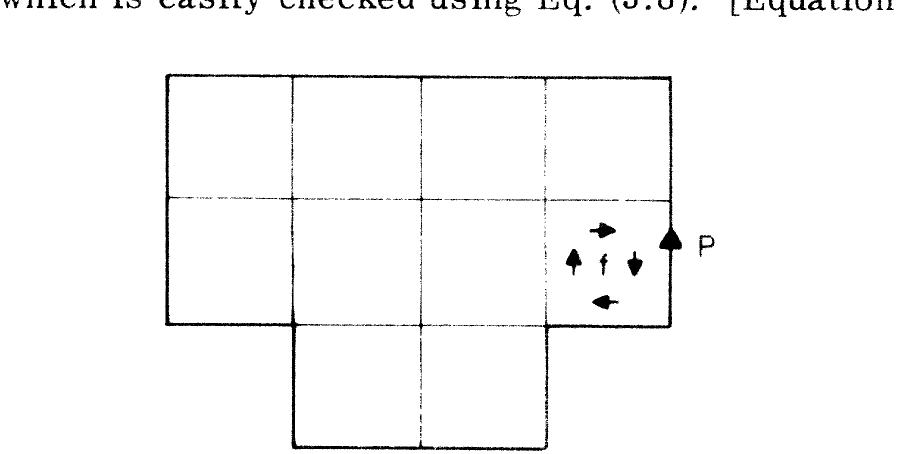
\includegraphics[width=0.5\textwidth]{fig10}
  \refstepcounter{figure}%
  \caption*{Fig. 10. Filling of enclosed area of path $P$ by elementary
    squares.}
  \label{fig:10}
\end{figure}

This is the result promised in Sec.~\ref{sec:binding}:  The gauge-field
average $I_{\theta}(P)$ behaves as
$\exp[-A\,(\ln g^{2})/a^{2}]$, i.e., exponentially in the area enclosed
by $P$.  Hence, according to the arguments of Sec.~\ref{sec:binding},
quark paths will not separate macroscopically, and there will be no
quarks among the final-state particles.

Consider higher-order terms in the expansion of $I_{\theta}(P)$ for
given $P$.  There are many such terms because there are many surfaces
with boundary $P$.  In particular, there are many ways to combine subsets
of $f$'s to add to zero so such subsets can be added to any minimal sum
of $f$'s which forms a surface with boundary $P$.  The simplest example
of a set of $f$'s which add to zero are the set of $f$'s corresponding
to the six faces of a unit cube.  Written out, this gives
\begin{equation}
\begin{split}
&f_{\mu\nu}(n)+f_{\mu\nu}(n+\hat\mu)+f_{\mu\nu}(n+\hat\nu)\\
&\qquad + f_{\mu\rho}(n)+f_{\rho\mu}(n+\hat\mu)+f_{\mu\rho}(n+\hat\rho)=0,
\end{split}
\label{eq:4.6}
\end{equation}
which is easily checked using Eq.~\eqref{eq:3.8}.  [Equation
\eqref{eq:4.6} is the lattice analog of the equation
$\epsilon_{\mu\nu\rho\sigma}\partial_{\rho}F_{\mu\nu}(x)=0$.]

Let $A(P)$ be the minimal area as defined above enclosed by $P$.  Since
one can place a unit cube anywhere on this minimal area, it means that
there are roughly $A(P)/a^{2}$ more terms of order $g^{-2(n+1)}$ in the
expansion of $I_{\theta}(P)$ than there are terms of order $g^{-2n}$.
[One can place unit cubes anywhere in space, not just on the minimal
surface; but when one divides $I_{\theta}(P)$ by $Z$ all disconnected
terms cancel, as usual.]  This suggests that the $1/g^{2}$ expansion is
not very useful in the limit $A(P) \to \infty$, which is the limit of
interest for quark binding.  However, experience with related problems
suggests that $I_{\theta}(P)$ is not the appropriate quantity to expand;
instead one should try writing
\[
I(P) = Z^{-1}I_{\theta}(P) = (g^{-2})^{A(P)/a^{2}}e^{-c(P,g^{2})}
\]
and expand $c(P,g^{2})$ in powers of $g^{-2}$ instead.  One would expect
$c(P,g^{2})$ to be dominated by a term proportional to $A(P)$, say
\[
c(P,g^{2}) = A(P)f(g^{-2}) + \order{P}
\]
(where $P$ is the length of the path $P$).  The crucial question is the
nature of the series for $f(g^{-2})$.  Past experience with similar types
of expansions (namely, the high-temperature expansions of statistical
mechanics:  see, e.g., Ref.~13) suggests that $f(g^{-2})$ will have a
convergent expansion at least for $g^{-2}$ less than a critical value
$g_{c}^{-2}$.  However, no calculations have been done in the
gauge-field theory for $f(g^{-2})$ as yet.

Consider the complete expansion of $I(P)$.  Each nonzero term in the
expansion corresponds to a surface with perimeter $P$.  The complete
expansion corresponds to a sum over all possible surfaces with given
perimeter $P$.  ``All possible'' surfaces include surfaces which
intersect themselves (to take into account terms where a given
$f_{\mu\nu}$ appears several times in the sum
$\sum f_{\mu\nu} + f_{\mu\nu'} + \cdots$).  There is a weight factor for
each surface, aside from the power of $g^{-2}$ determined by the area of
the surface.  For a simple surface, the weight factor is 1; the weight is
more complicated for self-intersecting surfaces.

Thus, the strong-coupling expansion for the current-current propagator
has the same general structure as in string models of hadrons.  One is
actually dealing here with a double expansion.  An expansion in the
coefficient $\kappa$ (appearing in the Dirac field action) was needed to
define quark loops on the lattice; the sum of the $\kappa$ expansion is a
sum over all possible quark loops.  The $g^{-2}$ expansion is needed to
define surfaces filling in the quark loops.  The sum of the $g$ expansion
is a sum over all such surfaces.  This is precisely the structure
appearing in string models:  combined sums over quark loops and
interpolating surfaces.  However, the loops and surfaces of the
gauge-field theory are defined on a lattice whereas the loops and
surfaces of the string models are defined on a continuum.  It may not be
easy to derive quantitative relations between the two types of surfaces.

% =====================================================================
%  Section V. Weak-Coupling Approximation
% =====================================================================
\section{WEAK-COUPLING APPROXIMATION}\label{sec:weak}

The weak-coupling approximation will be discussed briefly, leaving many
questions open.  Only the pure gauge field will be discussed.  Consider
again the expression
\begin{equation}
Z_{\theta}(P) = \prod_{n,\mu\nu}\int\ddth{\mu\nu}
  \exp\!\Bigl[i\sum_{P}(\pm)\thl{\mu\nu}
    +\frac{1}{2g^{2}}\sum_{n,\mu\nu}
      \bigl(1-\tfrac{1}{2}\bigl(e^{if_{\mu\nu}(n)}+e^{-if_{\mu\nu}(n)}\bigr)\bigr)\Bigr].
\label{eq:5.1}
\end{equation}

Suppose the integration variables were $f_{\mu\nu}$ rather than
$\thl{\mu\nu}$.  For small $g$, only small values of $f_{\mu\nu}$ would
be important in the integral, in order that
$\exp[(1/2g^{2})\cos f_{\mu\nu}]$ be near its maximum value 1.  One
would then expand:
\begin{equation}
\frac{1}{2g^{2}}\bigl(1-\cos f_{\mu\nu}\bigr)
  \approx \frac{1}{4g^{2}}f_{\mu\nu}^{2}+\cdots .
\label{eq:5.2}
\end{equation}
With this approximation one could extend the limits of integration on
$f_{\mu\nu}$ from $\pm\pi$ to $\pm\infty$, with negligible error; one
would then have a set of Gaussian integrals to evaluate.

In practice the integration variables are the $\thl{\mu\nu}$, not the
$f_{\mu\nu}$.  However, one can make a change of variable from the
$\thl{\mu\nu}$ to the $f_{\mu\nu}$.  It is not possible to eliminate all
the $\thl{\mu\nu}$ by this transformation, and not all the variables
$f_{\mu\nu}$ are independent.  Nevertheless, the transformation is
sufficient to make $I_{\theta}(P)$ calculable for small $g^{2}$.

To make the change of variables precise, consider a system of finite
size ($|n_{0}|,|n_{1}|,|n_{2}|,|n_{3}| \le N$) with periodic boundary
conditions.  Then one can change variables from the $\thl{\mu\nu}$ to a
subset of the $f_{\mu\nu}$ plus some gauge transformation variables
$\varphi_{n}$, plus four extra variables $\xi_{\mu\nu}$, as follows:

\emph{(i)}  For $n$ with $n_{0} < N$, $\thl{\mu\nu}$
($\mu=1,2,3$) is replaced by $f_{\mu\nu}$.  For $\thl{0\mu}$, one writes
\begin{equation}
\thl{0\mu} \to f_{0\mu},
\label{eq:5.3}
\end{equation}
and replaces $\thl{0\mu}$ by $\varphi_{\mu}$.  This is the essence of the
transformation from $\thl{\mu\nu}$ to $f_{\mu\nu}$ for $\mu \ne 0$ and
from $\thl{0\mu}$ to $\varphi_{\mu}$.  To complete the transformation one
must discuss the surface $n_{0}=N$.

\emph{(ii)}  For $n_{0}=N$, $n_{1}<N$, and $n_{2}$ and $n_{3}$ arbitrary,
$\thl{\mu\nu}(\mu,\nu\in\{1,2,3\})$ is replaced by $f_{\mu\nu}$;
$\thl{0\mu}$ is replaced by $\varphi_{\mu}$, with
\begin{equation}
\thl{0\mu}(n) = \varphi_{\mu}(n) + i\,\text{(linear combination of $f_{\mu\nu}$)}.
\label{eq:5.4}
\end{equation}

\emph{(iii)}  For $n_{0}=n_{1}=N$, $n_{2}<N$, and $n_{3}$ arbitrary,
$\thl{\mu\nu}(\mu,\nu\in\{2,3\})$ is replaced by $f_{\mu\nu}$;
$\thl{0\mu}$ is replaced by $\varphi_{\mu}$, with
$\thl{0\mu}=f_{0\mu}-\varphi_{\mu}$.

\emph{(iv)}  For $n_{0}=n_{1}=n_{2}=N$, and $n_{3}<N$,
$\thl{\mu\nu}(\mu=3)$ is replaced by $f_{3\nu}$; $\thl{0\mu}$ by
$\varphi_{\mu}$, where $\thl{0\mu}=\varphi_{\mu}-\varphi_{\mu}$.

\emph{(v)}  For $n_{0}=n_{1}=n_{2}=n_{3}=N$ one writes
$\thl{\mu\nu}=\xi_{\mu\nu}$ with $\xi_{\mu\nu}$ being the new variables.
One also sets $\varphi_{n}=0$ for this value of $n$.

The variables $f_{\mu\nu}$ which are not integration variables (for
example, $f_{\mu\nu}$ with $\mu\ne0$ and $\nu\ne0$, for $n$ with
$n_{0}<N$) can be expressed in terms of the independent $f_{\mu\nu}$
variables using Eq.~\eqref{eq:4.6}; neither the $\varphi_{n}$ nor
$\xi_{\mu\nu}$ appear in these expressions.

When an arbitrary $\thl{\mu\nu}$ is expressed in terms of the new
independent variables, one finds ($\xi_{\mu\nu}$ is present only if
$n_{0}=N$):
\begin{equation}
\begin{split}
\thl{\mu\nu}(n) = f_{\mu\nu}(n) &+ \text{(gauge-transformation terms)}\\
 &+ \text{(linear combination of $f_{\mu\nu}$)},
\end{split}
\label{eq:5.5}
\end{equation}
i.e., the $\varphi$ variables define a gauge transformation and $f$
represents a translation of some of the $\theta$'s.  It is easily
verified that the integrand of $Z_{\theta}(P)$ involves only the $f$'s:
It is independent of both the $\varphi$'s and $\xi_{\mu\nu}$ (the latter
does not appear because any closed path $P$ has as many
$-\thl{\mu\nu}$ terms as $+\thl{\mu\nu}$ terms on the sublattice
$n_{0}=N$).  Hence the $\varphi_{n}$ and $\xi_{\mu\nu}$ integrations can
be computed trivially.  The integrations are nontrivial because of the
constraint~\eqref{eq:4.6}.

What one wants to accomplish is to reduce the lattice theory for small
$g$ to something like a conventional free gauge-field theory.  This
means restoring the $\thl{\mu\nu}$ as the integration variables, but
with infinite limits of integration, and with a gauge-fixing term
included.  Suppose, for example, one starts with
\begin{equation}
\begin{split}
Z_{\theta}'(P) = \prod_{n,\mu\nu}\int\ddth{\mu\nu}\,
  \exp\!\Bigl[i\sum_{P}(\pm)\thl{\mu\nu}
    &+\frac{1}{2g^{2}}\sum_{n,\mu\nu}
      \bigl(1-\tfrac{1}{2}\bigl(e^{if_{\mu\nu}(n)}+e^{-if_{\mu\nu}(n)}\bigr)\bigr)\\
    &-\frac{\alpha}{2}\sum_{n}\bigl(\nabla_{\mu}A_{\mu}(n)\bigr)^{2}\Bigr],
\end{split}
\label{eq:5.6}
\end{equation}
where the $\alpha$ term is a lattice version of a
$(\nabla_{\mu}A_{\mu})^{2}$ gauge-fixing term.  This integral can be
computed by explicit Gaussian integration methods rather more easily
than the $f_{\mu\nu}$ integrations for $I_{\theta}(P)$.  In addition,
$I_{\theta}(P)$ can also be reduced to an integral over a subset of the
$f_{\mu\nu}$, using the same change of variables as for $I_{\theta}(P)$.
The result is different in this case due to the $\alpha$ term which
couples the $\varphi$'s to the $f$'s; also there is no convergence
factor for the $\xi$ integration.  To make $I_{\theta}'(P)$ well defined
and equal to $I_{\theta}(P)$, one must (a) put in a convergence factor
for the $\xi$ integral, i.e., a term $-\tfrac{1}{2}\alpha(\nabla_{\mu}A_{\mu})^{2}$, and
(b) add a quadratic form in the $\xi$'s to compensate for the result of
the $\xi$ integration of the gauge-fixing term.  The author has not
carried through this calculation; but since the net result is still that
$Z_{\theta}(P) = I_{\theta}'(P)$ is a Gaussian integration in the
$\theta$'s, the result will presumably be similar to the conventional
free-field calculation reported in Sec.~\ref{sec:binding}.

% =====================================================================
%  Section VI. Phase Transitions
% =====================================================================
\section{PHASE TRANSITIONS}\label{sec:phases}

In the strong-coupling limit ($g\to\infty$, $\kappa\to0$) the gauge
theory is far from being Lorentz-invariant.  More precisely, since the
action was defined on a Euclidean metric, it is Euclidean invariance that
is missing.  In the strong-coupling limit, vacuum expectation values
decrease rapidly at separations of only a few lattice sites (there is a
factor $g^{-2}$ or $\kappa$ or both for each unit lattice spacing of
separation).  This corresponds to the existence of masses much larger
than the cutoff.  [The usual rule is that if a propagator falls as
$e^{-\xi x}$ for $x$ large then the lowest mass intermediate state
contributing to the propagator has mass $1/\xi$.  If the propagator
behaves as $g^{-2x/a}$ for distances $x=na$, then the corresponding mass
is $2(\ln g)/a$.  This is larger than the cutoff momentum $\pi/a$ if $g$
is large.]

Thus, one is interested in practice in values of $g$ and $\kappa$ such
that the correlation length $\xi$ is much larger than the lattice
spacing $a$, in order that the corresponding mass is much less than the
cutoff.  One knows from statistical mechanics that large correlation
lengths are associated with second-order phase transitions (critical
points).  Thus one seeks special values $g_{c}$ and $\kappa_{c}$ for $g$
and $\kappa$ at which there is a phase transition.

It has already been argued that there are two distinct phases for the
gauge field, a strong-coupling phase for large $g$ which binds quarks,
and a weak-coupling phase for small $g$ which does not bind quarks.  The
arguments given neglected quark vacuum loops, which is reasonable if
$\kappa$ is small.  There should be a transition between these two
phases which would occur at a critical value $g_{c}$ for any $g$ and any
small value of $\kappa$.  This is one possible phase transition; it is
this transition which was discussed in Sec.~\ref{sec:binding}.  But, as
will be argued below, this is probably a first-order transition rather
than second order.

Suppose one wishes to construct a model of strong interactions using the
lattice theory of this paper with the gauge group separate from ordinary
SU(3)$\times$SU(3) symmetry.  Then the gauge fields would all be
SU(3)$\times$SU(3) singlets, while the quark fields would carry
SU(3)$\times$SU(3) quantum numbers as well as gauge-group quantum
numbers.  A little thought shows that in the strong-coupling limit
($g\to\infty$, $\kappa\to0$), SU(3)$\times$SU(3) is an exact symmetry
rather than a spontaneously broken symmetry.  Varying $g$ does not change
this situation; so one must hope that by increasing $\kappa$ one can
change the exact SU(3)$\times$SU(3) into broken SU(3)$\times$SU(3).  If
this does not work one is free to introduce additional terms into the
quark field action in hopes of forcing a spontaneous breaking of
SU(3)$\times$SU(3).  Suppose, for simplicity, that SU(3)$\times$SU(3)
can be broken by increasing $\kappa$.  Then there will be a phase
transition at a critical value $\kappa_{c}$ for $\kappa$ where one changes
from exact SU(3)$\times$SU(3) to spontaneously broken
SU(3)$\times$SU(3).  If this transition is a second-order transition then
there will be a large correlation length for $\kappa$ near $\kappa_{c}$;
in this case the theory might be a realistic model of broken
SU(3)$\times$SU(3) for $\kappa$ slightly greater than $\kappa_{c}$ (with
$g$ large enough to maintain quark binding).

In summary, the transition of real interest is a transition in $\kappa$
(or some other parameter introduced into the quark action) rather than
$g$.

Apart from special limits ($g\to\infty$ and $\kappa\to0$, or $g$ small)
it is very difficult to solve the lattice theory.  It is especially
difficult to solve the lattice theory near a critical point with a large
correlation length.  Various methods have been developed by statistical
mechanicians to deal with this problem.  In the remainder of this section
these methods will be discussed briefly.  There are essentially three
approaches to consider:  (1) mean-field techniques, (2) series
expansions, and (3) the renormalization-group approach.

Mean-field techniques${}^{15}$ are the simplest and crudest methods for
studying a critical point; invariably they are the methods one uses
first in studying a new situation.  They are used to determine if there
is a phase transition, whether it is first or second order, and to give
rough estimates of the behavior near the transition.  None of the
results of a mean-field calculation are entirely trustworthy.  Examples
of mean-field calculations will be given later.

An example of a series expansion would be the expansion of the
current-current propagator for small momentum (momentum $\ll 1/a$) in
powers of $g$ and $\kappa$, to high order in $g^{-2}$ and $\kappa$.  One
then uses Pad\'e-approximant techniques to look for singularities in
either $g$ or $\kappa$ that would be associated with a mass approaching
0.  In simple statistical-mechanical problems one can generate 12 terms
or so in analogous expansions.  The expansion for the lattice theory of
this paper is more complicated, but one could hope to generate maybe 6
or 7 orders with some practice.  Series expansions require considerably
more effort than mean-field calculations; they apply mainly to
propagators, being very awkward to perform on three- and four-point
functions, and one must have a clear idea of what one is trying to learn
before attempting such calculations.  See Ref.~16 for one of the best
series-expansion formalisms; see Ref.~13 for a general review.

The renormalization-group approach is potentially the most powerful and
accurate method for studying lattice theories near a critical point, but
at present the renormalization-group techniques are too limited in scope
to be applicable to the present problem.  See Refs.~6 and~17.

Return to mean-field ideas.  The prototype mean-field calculation is a
calculation of the magnetization as a function of the external field for
an Ising ferromagnet.  Let $s_{n}$ be the spin at site $n$ with values
$\pm 1$ only; let the interaction be
\begin{equation}
A = K\sum_{n,\mu}s_{n}s_{n+\hat\mu} + h\sum_{n}s_{n},
\label{eq:6.1}
\end{equation}
where $K$ is related to the spin-spin coupling and $h$ is proportional
to the external field.  Then
\begin{equation}
M = Z^{-1}\Bigl(s_{0}\exp\Bigl[K\sum_{n,\mu}s_{n}s_{n+\hat\mu}
    + h\sum_{n}s_{n}\Bigr]\Bigr),
\label{eq:6.2}
\end{equation}
where $(\ )$ means a sum over all configurations of all spins, and
\begin{equation}
Z = \sum\exp\Bigl[K\sum_{n,\mu}s_{n}s_{n+\hat\mu}
    + h\sum_{n}s_{n}\Bigr].
\label{eq:6.3}
\end{equation}

In the mean-field approximation, one assumes that the spins
$s_{n,\hat\mu}$, coupled to $s_{0}$, can be replaced by their average
value $M$.  As a result, the formula for $M$ simplifies to a sum over
$s_{0}$ only, namely
\begin{equation}
M = Z_{0}^{-1}\sum_{s_{0}=\pm 1}s_{0}\exp\bigl[(2dKM+h)s_{0}\bigr],
\label{eq:6.4}
\end{equation}
with $d$ being the dimensionality (3 usually) and
\begin{equation}
Z_{0} = \sum_{s_{0}=\pm 1}\exp\bigl[(2dKM+h)s_{0}\bigr].
\label{eq:6.5}
\end{equation}
The result is
\begin{equation}
M = \tanh(2dKM+h).
\label{eq:6.6}
\end{equation}
If $2dK<1$ this equation has a unique solution for $M$ as a function of
$h$; in particular, $M=0$ for $h=0$.  For $2dK>1$ the solution is
multiple-valued; stability considerations show that one must choose a
solution with $M\ne0$ when $h=0$.

In this approximation one has actually replaced $\sum_{\mu}s_{n,\hat\mu}$
by $2dM$, which is a good approximation if $d$ is large.  This is
generally true of mean-field theories.

An analogous mean-field calculation can be performed for the lattice
gauge theory.  In this case a simple external field term has the form
\[
\frac{1}{g}\sum_{n,\mu}\bigl(e^{i\thl{0\mu}(n)}+e^{-i\thl{0\mu}(n)}\bigr)
\]
(this is to be added to the gauge-field action), and $M$ can be defined
to be the expectation value of $e^{i\thl{0\mu}}$.  The question is
whether $M$ is zero in the limit $h\to0$.  In the gauge-field theory
$e^{i\thl{0\mu}}$ couples to a product of three other exponentials; as a
mean-field approximation one replaces this product by $M^{3}$.  The
result of this is that
\begin{equation}
M = Z_{\theta}^{-1}\int\ddth{0\mu}\,e^{i\thl{0\mu}}
  \exp\bigl[2(d-1)M^{3}+h\bigl(e^{i\thl{0\mu}}+e^{-i\thl{0\mu}}\bigr)\bigr],
\label{eq:6.7}
\end{equation}
where $d$ is the space-time dimensionality,
\begin{equation}
Z_{\theta} = \int\ddth{0\mu}
  \exp\bigl[2(d-1)M^{3}+h\bigl(e^{i\thl{0\mu}}+e^{-i\thl{0\mu}}\bigr)\bigr],
\label{eq:6.8}
\end{equation}
The result of this is that
\begin{equation}
M = f\bigl[2(d-1)M^{3}+h\bigr],
\label{eq:6.9}
\end{equation}
where $f$ is a ratio of Bessel's functions.  If $g$ is large the
solution to this equation is unique and $M=0$ for $h=0$.  If $g$ is
small then there are solutions with $M\ne0$ for $h=0$, and stability
considerations show again that the $M\ne0$ solutions are preferred.

In the magnetic case, one finds that the spontaneous magnetization $M$
goes to zero for $2dK-1\to0$ [from Eq.~\eqref{eq:6.6}].  However, the
gauge-field case never has a solution for $h=0$ with $M$ small but
nonzero.  Thus there is a first-order transition at the value of $g$ for
which $M$ changes from zero to being nonzero.

A nonzero value of $M$ in the limit $h\to0$ means one has spontaneous
breaking of the gauge-field symmetry.  So for small $g$ the theory shows
spontaneous breaking.

A much more thorough discussion of the mean-field approximation has been
given by Balian, Drouffe, and Itzykson.${}^{17}$  A Hamiltonian
formulation of the lattice gauge theory has been given by Kogut and
Susskind.${}^{18}$  A clear review of quark confinement in the lattice
theory is given in Ref.~20.  Another formulation of the connection
between strongly coupled gauge theories and string models is given in
Ref.~21.

% =====================================================================
%  Acknowledgments and References
% =====================================================================
\section*{ACKNOWLEDGMENTS}\label{sec:ack}

The author has benefited from conversations with many people in
developing and especially in understanding the lattice gauge theory.
Persons I am indebted to include J.~Bjorken, R.~P.~Feynman, M.~E.~Fisher,
D.~Gross, J.~Kogut, L.~Susskind, T.-M.~Yan, and members of a seminar at
Orsay.

\vspace{4mm}

\begin{center}
\footnotesize
\begin{minipage}{0.93\textwidth}
\raggedright
${}^{*}$Work supported in part by the National Science Foundation.

\begin{enumerate}[leftmargin=1.6em,itemsep=1pt,parsep=0pt,topsep=2pt]
\item See, e.g., J.~M. Cornwall and R.~E. Norton, Phys. Rev. D \textbf{8}, 3338 (1973); R.~Jackiw and K.~Johnson, \emph{ibid.} \textbf{8}, 2386 (1973); J.~Kogut and L.~Susskind, \emph{ibid.} \textbf{9}, 3501 (1974); D.~Amati and M.~Testa, Phys. Lett. \textbf{48B}, 227 (1974); G.~'t~Hooft, Nucl. Phys. B (to be published); P.~Olesen, Phys. Lett. \textbf{50B}, 255 (1974); A.~Chodos, R.~L.~Jaffe, K.~Johnson, C.~B.~Thorn, and V.~F.~Weisskopf, Phys. Rev. D \textbf{9}, 3471 (1974).
\item J.~Schwinger, Phys. Rev. \textbf{125}, 397 (1962); \textbf{128}, 2425 (1962).
\item J.~H. Lowenstein and J.~A. Swieca, Ann. Phys. (N.Y.) \textbf{68}, 172 (1971).
\item A.~Casher, J.~Kogut, and L.~Susskind, Phys. Rev. Lett. \textbf{31}, 792 (1973); Phys. Rev. D \textbf{10}, 732 (1974).
\item A.~Suri, Ph.D. thesis, Cornell University, 1969 (unpublished).
\item K.~G. Wilson and J.~Kogut, Phys. Rep. \textbf{12C}, 75 (1974).
\item S.~Coleman and E.~Weinberg, Phys. Rev. D \textbf{7}, 1888 (1973).
\item Y.~Nambu, in \emph{Symmetries and Quark Models}, proceedings of the International Conference on Symmetries and Quark Models, Wayne State University, 1969, edited by Ramesh Chand (Gordon and Breach, New York, 1970); L.~Susskind, Nuovo Cimento \textbf{69A}, 457 (1970); G.~Konisi, Prog. Theor. Phys. \textbf{48}, 2008 (1972); P.~Goddard, J.~Goldstone, C.~Rebbi, and C.~B.~Thorn, Nucl. Phys. \textbf{B56}, 109 (1972); J.-L.~Gervais and B.~Sakita, Phys. Rev. Lett. \textbf{30}, 716 (1973); S.~Mandelstam, Nucl. Phys. \textbf{B64}, 205 (1973).
\item R.~P. Feynman, Phys. Rev. \textbf{80}, 440 (1950).
\item See, e.g., E.~S. Abers and B.~W. Lee, Phys. Rep. \textbf{9C}, 1 (1973).
\item See, e.g., F.~A. Berezin, \emph{The Method of Second Quantization} (Academic, New York, 1966), pp.~52ff.
\item K.~G. Wilson, Phys. Rev. D \textbf{6}, 419 (1972).
\item M.~E. Fisher, Rep. Prog. Phys. \textbf{30}, 615 (1967).
\item For the relation of relativistic field theory to critical points see Ref.~6, Sec.~X, and references cited therein.  For a review see R.~Brout, \emph{Phase Transitions} (Benjamin, New York, 1965), p.~8.
\item D.~Jasnow and M.~Wortis, Phys. Rev. \textbf{176}, 739 (1968).
\item K.~G. Wilson, Carg\`ese (1973) Lecture Notes, in preparation.
\item R.~Balian, J.~M. Drouffe, and C.~Itzykson, Phys. Rev. D (to be published).
\item J.~Kogut and L.~Susskind, Phys. Rev. D (to be published).
\item K.~Wilson, Cornell Report No.~CLNS-271 (to be published in the proceedings of the conference on Yang-Mills Fields, Marseille, 1974).
\item H.~P. Nielsen and P.~Olesen, Nucl. Phys. \textbf{B61}, 45 (1973); L.~J.~Tassie, Phys. Lett. \textbf{46B}, 397 (1973).
\end{enumerate}
\end{minipage}
\end{center}


\end{document}
